\subsection*{Метод Монте-Карло}
\addcontentsline{toc}{subsection}{Метод Монте-Карло}

\textbf{Задание:}\\
Используя метод Монте-Карло, вычислить $\int_{0}^{1} \sin(\pi x) dx$. Проанализируйте, как зависит точность полученного результата от количества точек, использованных для получения оценки. Постройте график этой зависимости.\\

\textbf{Решение:}\\
Для начала стоить нарисовать график данной функции $\sin (\pi x)$ и сгенерировать $n$ штук случайных точек.  (Рисунок \ref{fig:monte_carlo_example})
\begin{figure}[h]
	\centering 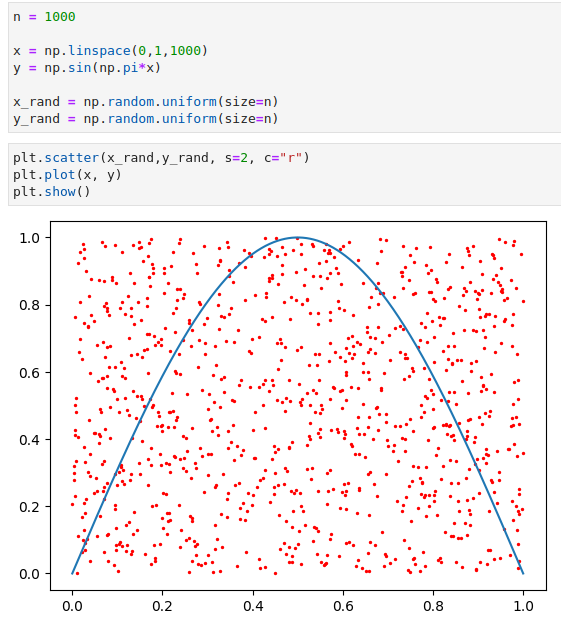
\includegraphics[scale=0.6]{monte_carlo_example}
	\caption{Пример применения метода Монте-Карло}
	\label{fig:monte_carlo_example}
\end{figure}

Далее остаётся просто посчитать то количество точек, которые попали под график и разделить их на общее количество сгенерированных точек.

\newpage

Данный алгоритм был реализован на языке программирования Python. (Рисунок \ref{fig:monte_carlo_code})
\begin{figure}[h]
	\centering 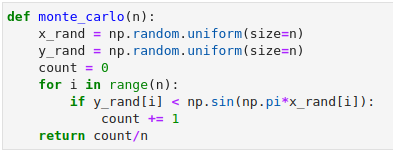
\includegraphics[scale=0.65]{monte_carlo_code}
	\caption{Реализация метода Монте-Карло для подсчёта интеграла}
	\label{fig:monte_carlo_code}
\end{figure}

Также была проанализирована зависимость между точностью результата и количеством сгенерированных точек. (Рисунок \ref{fig:monte_carlo_result})
\begin{figure}[h]
	\centering 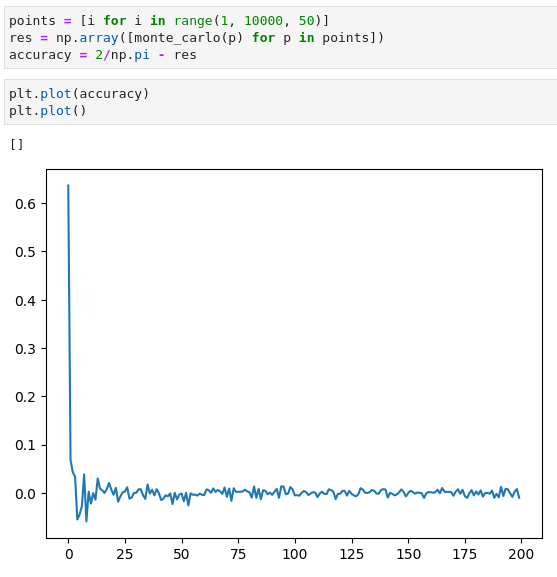
\includegraphics[scale=0.5]{monte_carlo_result}
	\caption{Зависимость точности результатов от количества точек}
	\label{fig:monte_carlo_result}
\end{figure}

Как можно видеть на графике, что чем больше количество сгенерированных точек, то тем точнее получается результат.